\documentclass[12pt]{article}

% Prevent words to overflow over the margin
% \sloppy  % Alternative command
\emergencystretch 3em

% Math
% the journal version already loads these packages
\usepackage{amsmath,amssymb,amsthm}
\renewcommand{\qedsymbol}{$\blacksquare$}

% Images and plots
\usepackage{subfig}
\usepackage{verbatim}
\usepackage{graphicx}
\graphicspath{ {images/} }
\usepackage{pgfplots}

\usepackage{mathtools}
\usepackage{enumitem}
\usepackage{multirow}
\usepackage{algorithm}% http://ctan.org/pkg/algorithms
\usepackage[noend]{algpseudocode} % Avoid "end" and make it look cleaner

\usepackage[margin=1in]{geometry}
% Tables
\usepackage{csvsimple}	% reading CSV files in tables
\usepackage{booktabs}   % Nicer Tables
\usepackage{adjustbox}  % To adjust table length
\usepackage{appendix}
\usepackage{multicol}
% Hyper-references
\usepackage{hyperref}


% Acronyms
\usepackage[xindy, acronyms]{glossaries}   % Glossaries and Acronyms
\makeglossaries

% Other 
\usepackage[textsize=tiny, color=blue!20]{todonotes}
\newcommand{\AAANote}[1]{\todo[inline, caption={}]{ Amirali: #1}}
\newcommand{\ColeNote}[1]{\todo[inline, caption={}]{ Cole: #1}}
\newcommand{\priv}{\text{IPT}}
\newcommand{\privuip}{\text{IPT}^\text{IP}}
\newcommand{\privlip}{\text{IPT}_\text{IP}}
\newcommand{\privsdp}{\text{IPT}^\text{SDP}}

% Definitions
% Stochastic optimization
\newcommand{\uncset}{{\mathcal{U}}}
\newcommand{\uMat}{\texttt{\textbackslash uMat}}

% Commands
\newcommand{\eg}{{\it e.g.}}
\newcommand{\ie}{{\it i.e.}}

% Sets
\newcommand{\ones}{\mathbf 1}
\newcommand{\reals}{{\mbox{\bf R}}}
\newcommand{\integers}{{\mbox{\bf Z}}}
\newcommand{\symm}{{\mbox{\bf S}}}  % symmetric matrices
\newcommand{\NPhard}{\mbox{$\mathcal{NP}$-hard}}  % symmetric matrices
\newcommand{\prob}{{\mathbf P}}
\newcommand{\distrib}{{\mathcal P}}
\newcommand{\identity}{I}
\newcommand{\tpose}{T}
\newcommand{\nullspace}{{\mathcal N}}
\newcommand{\range}{{\mathcal R}}
\newcommand{\Rank}{\mathop{\bf Rank}}
\newcommand{\Tr}{\mathop{\bf tr}}
\newcommand{\diag}{\mathop{\bf diag}}
\newcommand{\lambdamax}{{\lambda_{\rm max}}}
\newcommand{\lambdamin}{\lambda_{\rm min}}
\newcommand{\Expect}{{\mbox{\bf E}}}
\newcommand{\Co}{{\mathop {\bf Co}}} % convex hull
\newcommand{\dist}{\mathop{\bf dist{}}}
\newcommand{\epi}{\mathop{\bf epi}} % epigraph
\newcommand{\Vol}{\mathop{\bf vol}}
\newcommand{\dom}{\mathop{\bf dom}} % domain
\newcommand{\intr}{\mathop{\bf int}}
\newcommand{\dif}{\text{d}}
\newcommand{\sign}{\mathop{\bf sign}}
\newcommand{\round}{\mathop{\bf round}}
% \newcommand{\define}{\coloneqq}
\newcommand{\define}{=}
\newcommand{\defn}{\define}
\newcommand{\norm}[1]{\| #1 \|}
\renewcommand{\Re}{\reals}
\newcommand{\set}[2]{\{ #1 \mid #2 \}}

% Already defined commands in journal version

% Create theorems and other environments
\newtheorem{theorem}{Theorem}[section]  % Restart counter every section
\newtheorem{lemma}{Lemma}[section]  % Restart counter every section
\newtheorem{corollary}{Corollary}[theorem]  % Restart counter every theorem
\newtheorem{proposition}{Proposition}[section]
\newtheorem{assumption}{Assumption}[section]
\newtheorem{definition}{Definition}[section]
\newtheorem{example}{Example}[section]
\newtheorem{exercise}{Exercise}[section]
\newtheorem{remark}{Remark}[section]
\newtheorem{problem}{Problem}[section]



% Trees
\newcommand{\tree}{\mathcal{T}}

% Other
\newcommand{\tb}{\textbf}
\newcommand{\mr}{\mathbb{R}}
\newcommand{\mc}{\mathcal}
\newcommand{\sbs}{\subseteq}
\newcommand{\sps}{\supseteq}
\newcommand{\prf}{\textbf{\underline{Proof:}} }
\newcommand{\ans}{\textbf{\underline{Answer:}} }
\newcommand{\lma}{\textbf{\underline{Lemma:}} }

% Acronyms
\newacronym{IPT}{IPT}{Information Privacy Tradeoff Problem}
\newacronym{GIPT}{GIPT}{Generalized Information Privacy Tradeoff Problem}
\newacronym{KNAP}{KNAP}{Knapsack Problem}
\newacronym{MIP}{MIP}{Mixed Integer Program}
\newacronym{SOCP}{SOCP}{Second Order Cone Program}
\newacronym{LP}{LP}{Linear Program}
\newacronym{IP}{IP}{Integer Program}
\newacronym{poi}{poi}{Person of Interest}






\begin{document}



\title{Information Privacy Tradeoff}
\author{Cole Becker and Amir Aliddd}
\date{September 2022}
\maketitle

\section{Related Works}
\subsection{Differential Privacy}
\subsection{Knapsack Problem}
\subsection{Complexity}

\section{The Problem}
We consider the following decision problem, we denote \gls{IPT}
\paragraph{Input:}
Consider a dataset $\mc{D} = \{d_i\}_{i\leq m} \sbs \mr^n$ where $d_i \in \{0,1\}^n$, and denote $D\in \mr^{m\times n}$ as the matrix containing this data. We can imagine for example that $m$ is the number of people in the dataset, and $d_i\in \mr^n$ represents a binary feature vector of information on $n$ features for the $i$th person. In addition, you are given a non-negative weight vector $w\in \mr^n$ representing the relative importance of each the $n$ features, some number $r \in [0,1]$ and an index $k \in \{1,...,m\}$. Finally we also take in a non-negative number $l \in \mr$.
\paragraph{Question:}
Is there a way to select a subset of features of $d_k$, indexed by $x\in \{0,1\}^n$ such that $w^T x \geq l$ and the subset features of $d_k$ are shared by at least $rm$ people in the dataset ($d_k$ included). \tb{Note}: Throughout the entirety of this paper, we will assume $k = 0$ unless otherwise specified, and we will refer to $d_k$ as \gls{poi}.
\subsection{Motivation}
Suppose you are a company holding such a dataset $\mc{D}$ about various attributes of a large quantity of individuals. Some advertising company Ad.co comes to you, and wants to purchase the data of some individual $k$ to run some targeted advertising of their own. In order to convey which features they are most interested in knowing, or which features are most useful to their advertising campaign, they supply you with a weight vector $w$ which represents how much Ad.co values knowing each feature of individual $k$ in your dataset. However, as your company must comply with privacy regulations, you are not allowed to share too much information about individual $k$ which would distinguish them too much. Specifically, the features you reveal to Ad.co about individual $k$ must also be shared by $100 * r\%$ of the members of your dataset. Your task is to maximize the useful information you can share with Ad.co while satisfying the imposed privacy constraints.


\subsection{Formulation of \gls{IPT}}
Taking all the same inputs from the above problem, let us first define a helper matrix $K \in \mr^{m\times n}$ as
\begin{align*}
    K_{ij} = \begin{cases}
        0 & \text{ if } D_{ij} = D_{kj} = (d_k)_j\\
        1 & \text{ otherwise}
    \end{cases}
\end{align*} 
We note that \gls{IPT} can be reduced to the following non-convex optimization problem
\begin{equation}
	\label{eq:priv} 
    \tag{$\priv$} 
	\begin{array}{lll}
		\priv = & \underset{x}{\text{maximize}} & w^T x \\
		& \mbox{subject to} & ||K x||_{0}  \leq m(1-r) \\
        && x_i \in \{0,1\}
		\end{array}
\end{equation}
where the answer to the decision question is given by whether $\priv \geq l$. To see why the constraint in this problem is equivalent to the requirement that the subset $x$ of $d_k$'s features is shared by at least $rm$ people, note that  \[(Kx)_i = \begin{cases}
    0 & \text{ if } d_i \text{ shares the same } x \text{ features with } d_k \\
    > 0 & \text{ otherwise}
\end{cases}
\]
so the number of 0-elements in $Kx$ must be greater than $mr$ or equivalently, the number of non-zero elements must be less than $m(1-r)$ 

\subsection{Related Problem}
A closely related problem is the following problem is \gls{GIPT}
\[\text{GIPT} = \text{argmin}_k \ \priv_k\]
where $\priv_k$ represents the information privacy tradeoff of the $k$th individual in the dataset. We can think of the minimum over all such individauls as the most distinguishable/unique, or least anonymous individual. This is the individual for whom you can reveal the least information before they begin to be distinguishable from $r$\% of the dataset. 
In a closely related problem, we have 
\[\text{argmax}_k \ \priv_k\]
which can be thought of as the most anonymous and least unique individual in the dataset. 
\paragraph{20 Questions}
A simple way to think of this problem is as a game. Given a dataset of possible things to guess in a game of twenty questions (or people to learn information from), you would like to choose the least distinguishable individual to maximize the amount of guesses  \\
\tb{NOTE}: $\text{argmax}_k \ \priv_k$ isn't quite identical to 20 questions. What is the goal of twenty questions? The goal as a guesser is to reveal the features that on average leave the fewest members remaining. Here we are interested in privacy, so it would be more of a word producing game. We would want to produce a word such that on average, it is very anonymous. In other words, no matter what features you reveal, it doesn't narrow down your search very much. $\text{argmax}_k \ \priv_k$, means that you can reveal lots of features without narrowing the search down much. However think of the worst case scenario, in which there is one feature that such an individual has that she shares with nobody. This would make them distinguishable in a way, even if they were very anonymous with respect to their other features. So perhaps it isn't entirely obvious that $\text{argmax}_k \ \priv_k$ is the best metric for a 20 questions guessing game.

\section{Complexity of \gls{IPT}}
\begin{theorem}
    \gls{IPT} is NP-complete
\end{theorem}
\begin{proof}
    It is sufficient to show that \gls{IPT} $\in $ NP and that \gls{KNAP} $ \longrightarrow$  \gls{IPT}
    \begin{enumerate}
        \item \gls{IPT} $\in $ NP: Given a certificate solution $x^*$ to $\priv$, it is easy to check that the constraints are satisfied, and that $w^T x^* \geq l$
        \item \gls{KNAP} $ \longrightarrow$  \gls{IPT}: Consider the classic \gls{KNAP}:
        \\ \tb{Input:}
        \textit{$w \in \mr^n$ a weight vector of $n$ items, $p \in \mr^n$ a price vector for the items, $W\in \mr$ a weight capacity, and $P \in \mr$}
        \\ \tb{Question:}
        \textit{Is there a set of items of combined weight less than $W$ but with combined price greater than $P$?}
        \\~\\ 
        Using these inputs we will construct an instance of \gls{IPT} (Note we will assume for convenience that $W \in [0,1^Tw]$. If not we can define a new $W$ that is respective endpoint). To begin, set $m = 1+ 1^Tw$ and construct the following data matrix $D \in \mr^{m\times n}$ by the following procedure:
        \begin{enumerate}
            \item Set the first row of $D$ to a row of all $0$s
            \item For each weight $w_i$, $i\in\{1,...,n\}$ add $w_i$ copies of the one hot encoded row vector $e_i$. As an example:
            \[w = [3,1,2,1] \implies D = \begin{bmatrix}
                0&0&0&0 \\
                1&0&0&0 \\
                1&0&0&0 \\
                1&0&0&0 \\
                0&1&0&0 \\
                0&0&1&0 \\
                0&0&1&0 \\
                0&0&0&1 
            \end{bmatrix}\]
            This is the data matrix $D$ we will consider. Note that the auxiliary matrix $K$ used in \gls{IPT} is identical to $D$ via the way we constructed it.
        \end{enumerate}
        In addition, set $r = 1 - W/m$ (whereby assumption on $W$ we have $r \in [0,1]$), $l = P$, $k = 1$ the first row, and $\bar{w} = p$, the information weighting vector. We now have an instance of \gls{IPT}. In terms of the \gls{KNAP} variables, the equivalent \gls{IPT} problem looks like the following:
        \begin{equation}
            \begin{array}{lll}
                \priv(\text{KNAP}) = & \underset{x}{\text{maximize}} & p^T x \\
                & \mbox{subject to} & ||D x||_{0}  \leq W \\
                && x_i \in \{0,1\}
                \end{array}
        \end{equation}
        Notice the problem construction requires a polynomial amount of operations, as the size of $D = n * (1+ 1^T w)$, and everything else requires an affine amount of operations.
        We would now like to show the following equivalence between the problems. 
        \[\text{\gls{KNAP}} \geq P \iff \text{IPT(KNAP)} \geq P\]
       (\underline{$\Longrightarrow$}): Consider a solution $\hat{x}\in \{0,1\}^n$ to \gls{KNAP} satisfying the weight constraints and with $p^Tx \geq P$. This same solution $\hat{x}$ will be feasible to IPT(KNAP). To see why, just note that $||Dx||_0 = w^Tx$ is equivalent to taking the sum of the weights, because the construction of $D$ and $x$ mean that $||Dx||_0 = 1^TDx$ and $1^TD = w$ by construction. \\
       (\underline{$\Longleftarrow$}): The backwards argument is similar, but we need to build back the weight vector $w$ from the matrix $D$. To do so we again note that $w = 1^TD$, and then the problem is identical to knapsack.
    \end{enumerate}
\end{proof}


\section{Bounds and Relaxations for \gls{IPT}}
\subsection{\gls{MIP} Bounds}
As written in its L-0 form, \gls{IPT} is not even a mixed-integer program. Here we investigate affine relaxations of the L-0 norm and possible interpretations.
\subsubsection{\gls{MIP} Upper Bound}
We write an IP relaxation of \gls{IPT} as the following problem
\begin{equation}
	\label{eq:privuip} 
    \tag{$\privuip$} 
	\begin{array}{lll}
		\privuip = & \underset{x\in\mr^n}{\text{maximize}} & w^T x \\
		& \mbox{subject to} & \mathbf{1}^TKx \leq m(1-r)\mathbf{1}^Tx \\
        && x_i \in \{0,1\}
		\end{array}
\end{equation}
Where we have $\priv \leq \privuip$. To see why we would like to show
\[x \text{ feasible to } \priv \implies x \text{ feasible to } \privuip.\]
Consider $x^*$ feasible to $\priv$. If $x^* =0$ then $x^*$ is clearly feasible to $\privuip$ as both constraints are trivially satisfied. Now suppose $x^*\neq 0$, we want to show that \[\frac{\mathbf{1}^TKx^*}{\mathbf{1}^Tx^*} \leq m(1-r),\] or equivalently, that $\frac{\mathbf{1}^TKx^*}{\mathbf{1}^Tx^*} \leq ||Kx^*||_0$. The key is to notice is that $(Kx^*)_i \leq \mathbf{1}^Tx^*$ for all $i\leq m$ due to the binary nature of the entries of $K$ and $x^*$, which means that 
\[\left(\frac{\mathbf{1}^TKx^*}{\mathbf{1}^Tx^*}\right)_i = 
\begin{cases}
    0 & \text{ if } (Kx^*)_i = 0 \\
    \leq 1 & \text{ otherwise}
\end{cases}
\]
from the above statement we have
\[\frac{\mathbf{1}^TKx^*}{\mathbf{1}^Tx^*} \leq ||Kx^*||_0\]
so $x^*$ is feasible to $\privuip$, and $\priv \leq \privuip$.
% and consider an indicator vector $y \in \mr^m$ with 
% \[y_i = \begin{cases}
%      1 & \text{ if } d_i \text{ shares the same } x \text{ features with } d_k \\
%     0 & \text{ otherwise.}
% \end{cases}
% \]
%  We want to ensure that $1^T y \geq rm$. However we claim that $\frac{1^T \bar{K}x}{1^Tx} \geq 1^T y$. To see why, note that $(\bar{K}x)_i$ counts the number of features out of $x$ that $d_i$ and $d_k$ share, so 
% \[\left(\frac{\bar{K}x}{1^T x}\right)_i = 
% \begin{cases}
%     1 & \text{ if } d_i \text{ shares the same } x \text{ features with } d_k \\
%     \in [0,1) & \text{ otherwise}
% \end{cases}\]
% Of course to be sure that at least $rm$ individuals share the same features as the $d_k$th individual, we can sum to get $\frac{1^T\bar{K}x}{1^T x} \geq 1^Ty \geq rm$, and we get the constraint in $\privl$. 


\subsubsection{\gls{MIP} lower bound}
Next consider the following linear integer program
\begin{equation}
	\label{eq:privlip} 
    \tag{$\privlip$} 
	\begin{array}{lll}
		\privlip & = \underset{x}{\text{maximize}} & w^T x \\
		&\mbox{subject to} & \mathbf{1}^TKx \leq m(1-r) \\
        && x_i\in \{0,1\}
		\end{array}
\end{equation}
To see why $\privlip \leq \priv$, we would like to show that 
\[x \text{ feasible to } \privlip \implies x \text{ feasible to } \priv.\]
Fix $x^*$ feasible to $\privlip$. Due to binary nature of $K$ and $x^*$, we know $Kx^*$ is a non-negative integer vector. This means $\mathbf{1}^TKx^* = ||Kx^*||_1$ and so we have \[ ||Kx^*||_0 \leq ||Kx^*||_1 = \mathbf{1}^T K x^* \leq m(1-r)\]
so $x^*$ is feasible to $\priv$, and $\privlip \leq \priv$

\subsubsection{Relation to \gls{KNAP}}
Succinctly, we have shown that \ref{eq:privlip} $\leq$ \ref{eq:priv} $\leq$ \ref{eq:privuip} due to the fact that for non-zero $x$, we have \[\frac{\mathbf{1}^TKx}{\mathbf{1}^Tx} \leq ||Kx||_0 \leq \mathbf{1}^TKx\]
However if we define $\alpha := \mathbf{1}^TK$, then we can interpret \ref{eq:privlip} as a knapsack problem, where each item in the knapsack corresponds to a feature in our dataset. In this way, we can interpret the $i$th item $\alpha_i$ as a collection of people with feature $i$ distinct from our choice user. In other words, the weight of each item $\alpha_i$ is the number of people with feature $i$ distinct. This means that for a chosen subset of items (or features) $x$ to put in our knapsack, we can interpret the total weight of each of these items $\alpha^T x = \mathbf{1}^TKx$, as the total number of people in our knapsack, where we count each person once for each distinct feature they have. This means if person $i$ has 4 distinct features from \gls{poi}, then they will be counted 4 times and provide a weight of 4 into the knapsack. As $(Kx)_i$ represents the number of unique features individual $i$ has from \gls{poi}, every person is added $(Kx)_i$ times to the bag. In other words, $(Kx)_i$ represents how many items individual $i$ is in out of the subset $x$. In this way, counting the number of "unique" people in our knapsack corresponds to counting the number of people with $\geq 1$ distinct feature from \gls{poi}, which is equivalent to $||Kx||_0$. To illustrate this, consider an example $K$, and feature vector $x$ 
\[K = \begin{bmatrix}
    0&0&0 \\
    1&0&0 \\
    1&1&0\\
    0&1&1
\end{bmatrix}, \quad x = [1,1,0]^T, \quad Kx = \begin{bmatrix}
    0\\1\\2\\1
\end{bmatrix}, \quad \alpha = \begin{bmatrix}
    2&2&1
\end{bmatrix}\]
Where we he have three individuals (call them A,B,C) aside from \gls{poi} (row 1) and three features. We can view the items in our knapsack $\alpha = \mathbf{1}^TK$ as the following objects (one for each of the three features).
\begin{figure}[H]
    \centering
    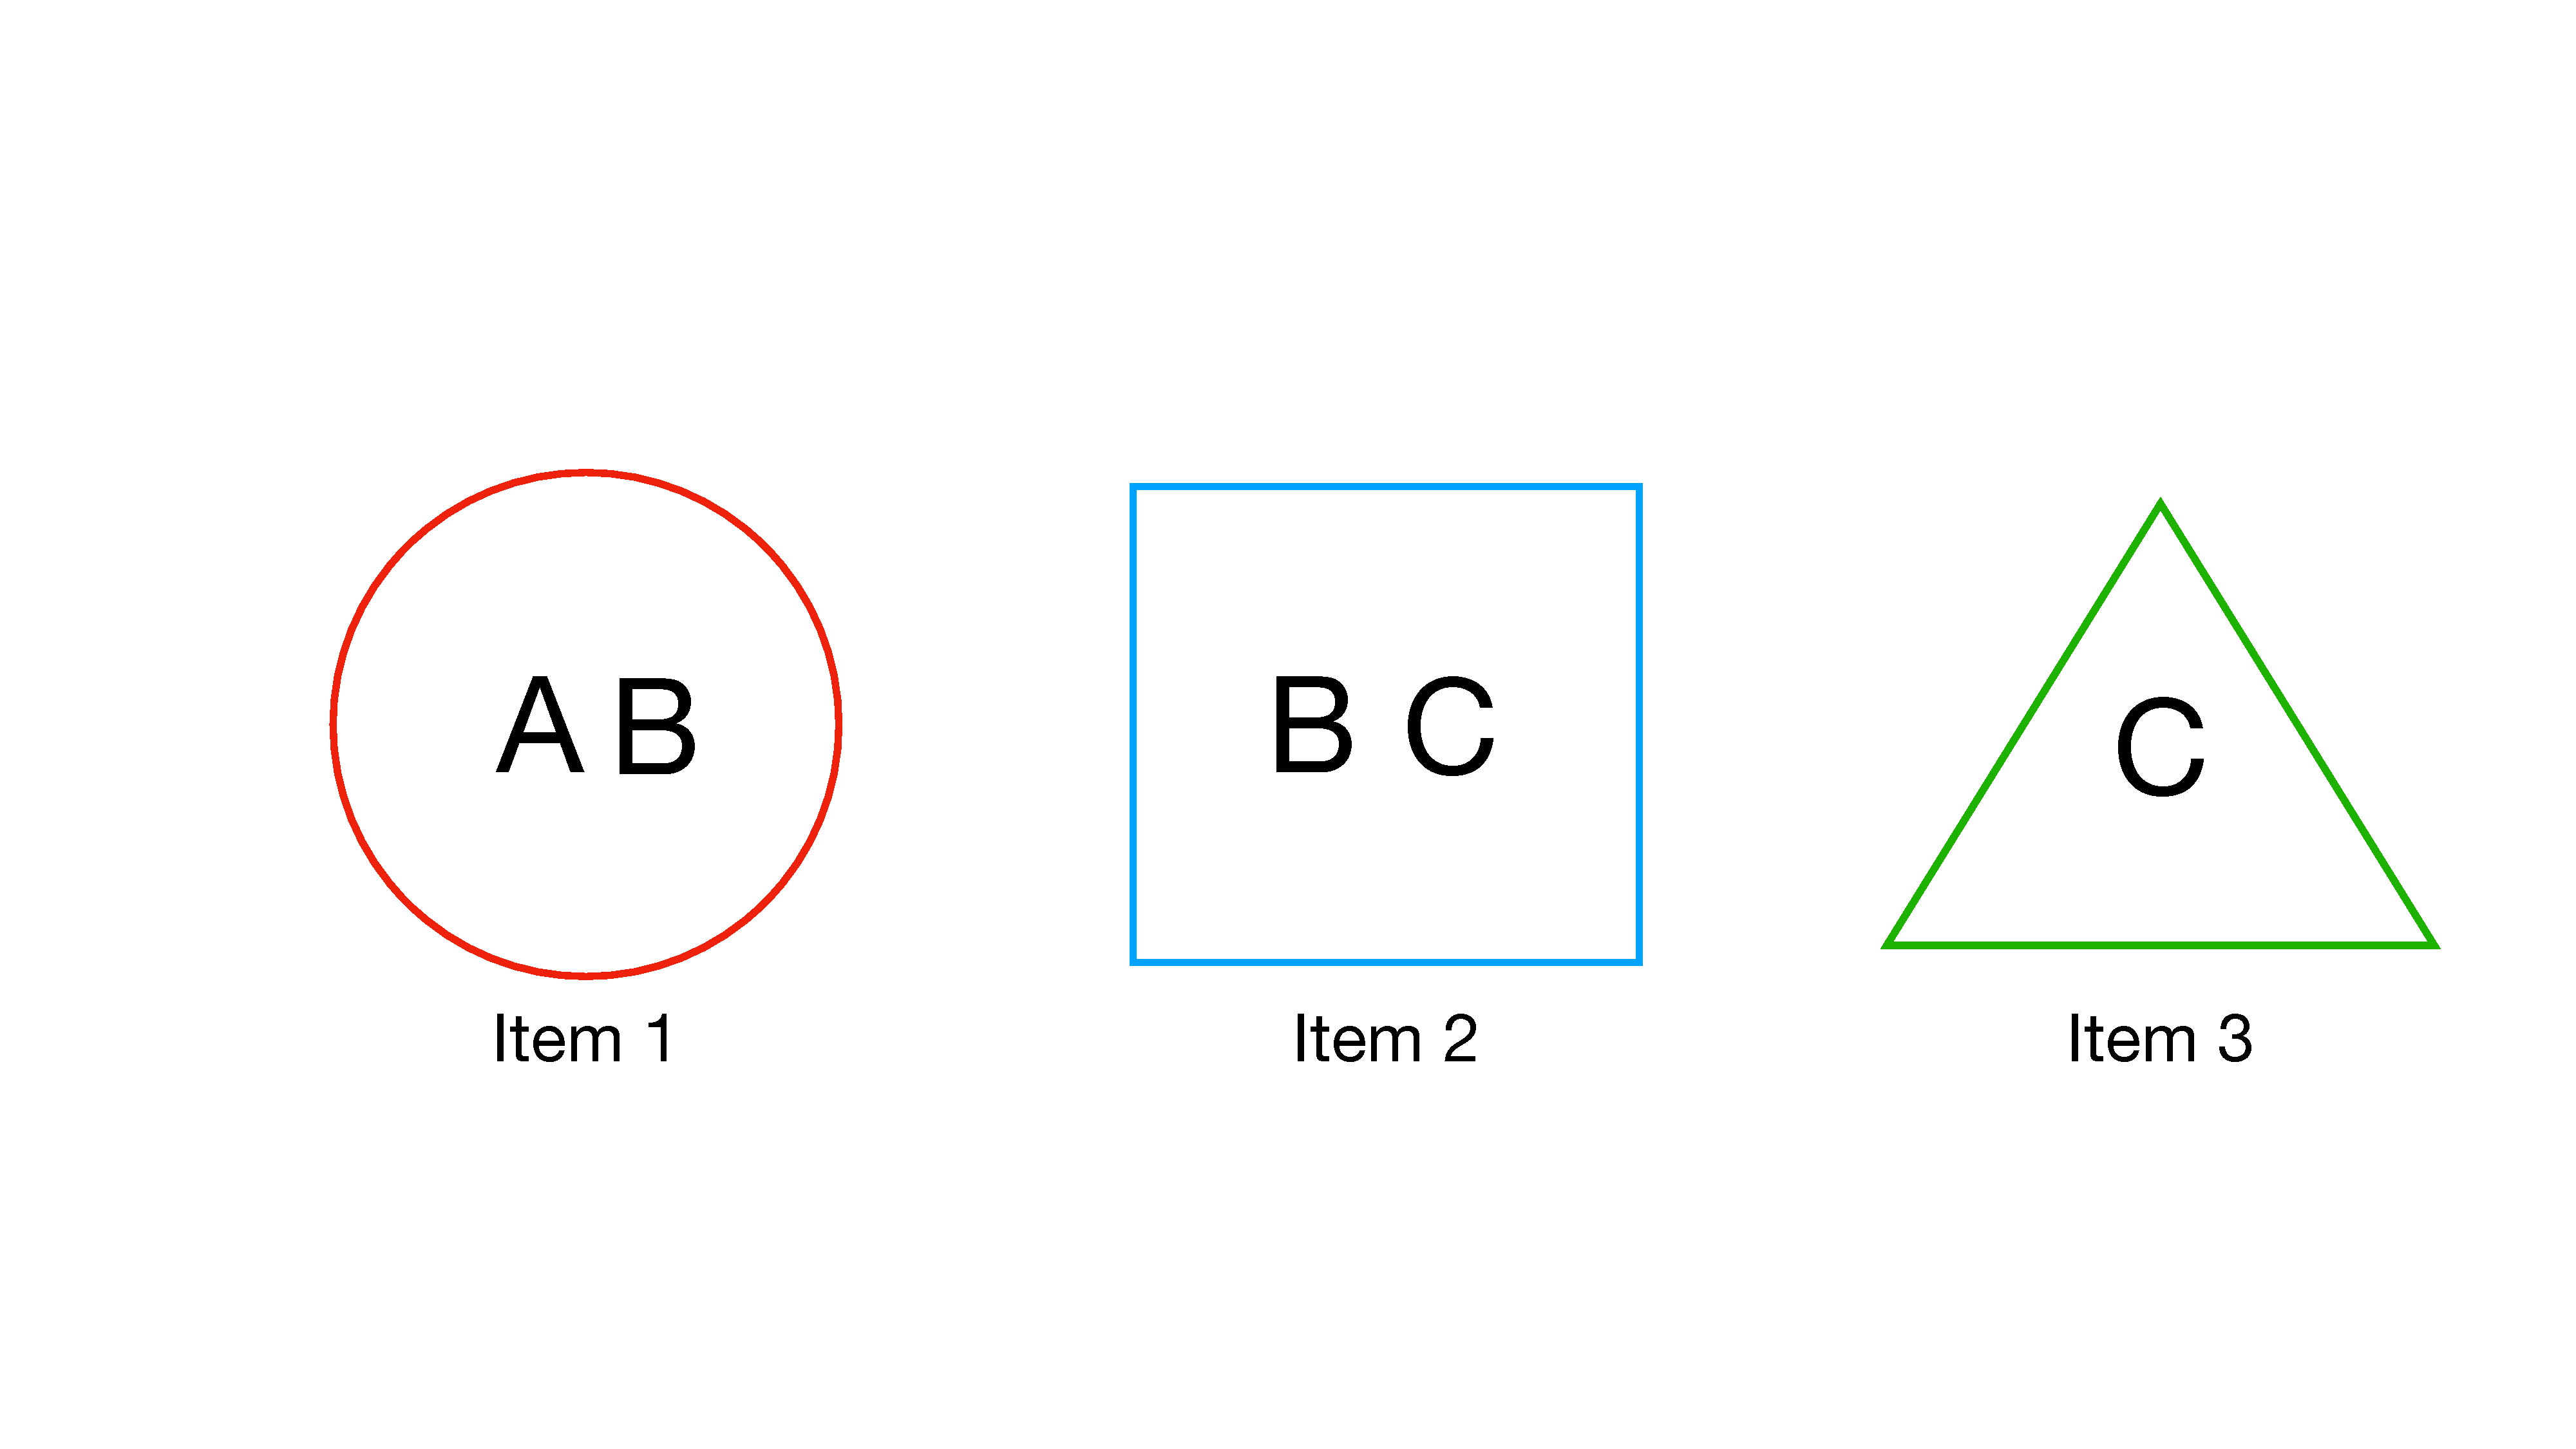
\includegraphics[width = 14cm]{images/knap_intuition.pdf}
    \label{fig:items}
\end{figure}
Here we only select the first two items $x = [1,1,0]^T$, so the weight of our knapsack $\mathbf{1}^TKx = \alpha^Tx = 4$. However, there are only three unique individuals in our knapsack, as we double count $B$. In order to only count $B$ once, we just take $||Kx||_0 = 3$ (i.e. count the number of non-zeros)
% The process of removing the duplicates, is equivalent to taking
% \[Kx = \begin{bmatrix}
%     0 \\1 \\2\\1
% \end{bmatrix} \to \begin{bmatrix}
%     0 \\1 \\1 \\1
% \end{bmatrix}\]
% To summarize we have 
% \begin{align*}
%     (Kx)_i &= \text{ number of distinct features of person $i$ from subset $x$} \\
%     \alpha_i = (\mathbf{1}^TK)_i &= \text{ number of }
% \end{align*}

\subsection{Convex Bounds}
\subsubsection{SDP Upper bound}
Consider the following SDP:
\begin{equation}
	\label{eq:privsdp} 
    \tag{$\privsdp$} 
	\begin{array}{lll}
		\privsdp = & \underset{x\in\mr^n}{\text{maximize}} & w^T x \\
		& \mbox{subject to} &  
        \begin{bmatrix}
            \begin{matrix}
                X
            \end{matrix}  & 
            \begin{matrix}
                Z
            \end{matrix} & x \\
            \begin{matrix}
                Z^T 
            \end{matrix} & 
            \begin{matrix}
                Y 
            \end{matrix} & y \\
            x^T & y^T & 1
        \end{bmatrix} \succeq 0\\
        && x_i = X_{ii}, \quad \forall i\leq n\\
        && y_j = Y_{jj}, \quad \forall j \leq m\\
        && \mathbf{1}^Ty \geq rm \\
        && 0 \leq x,y \leq 1
		\end{array}
\end{equation}
To see wh $\priv \leq \privsdp$, we would like to show that
\[x^* \text{ feasible to } \priv \implies \exists x,y,X,Z,Y \text{ feasible to }\privsdp\] 
Take $x^*$ feasible to $\priv$ and let $x = x^*$. Next define a vector $y \in \mr^n$ with each entry define as
\[y_i = \begin{cases}
    1 & \text{if } (Kx)_i = 0 \\
    0 & \text{otherwise}
\end{cases}\]
In other words, $y_i = 1$ if all subfeatures of individaul $i$ are shared with \gls{poi}. As $\mathbf{1}^Ty$ represents the number of individauls indistinguishable from \gls{poi}, clearly we will satisfy the constraint that $\mathbf{1}^Ty \geq rm$ by $x$ being feasible to $\priv$. As $x,y$ are also binary vectors, we satisfy that equality as well. Next define \[X = xx^T, \ Z = xy^T, \ Y = yy^T\]
and by Schur's complement, we satisfy the psd constraint, and the equality constraints. So we have feasiblity to $\privsdp$. Note that of course we can add on a the linear constraint from the MIP upper bound $\mathbf{1}^TKx \leq m(1-r)\mathbf{1}^Tx$ to get a tighter SDP relaxation.

\subsubsection{Greedy Lower Bound}
    Define $\bar{K} = 1 - K$ as the matrix with the entries in $K$ flipped. Now for any column $\bar{K}_i$ of matrix $\bar{K}$, define its value \[v(\bar{K}_i) = (1^T \bar{K}_i) w_i\] and order the columns from largest to smallest value, then perform a greedy selection algorithm by selecting the columns with the largest value up until the privacy constraint is violated. The idea is we both want to select columns which are weighted highly and who share features with the $k$th column.  Note that we can always rewrite $\mathbf{1}^T\bar{K} = m - \mathbf{1}^TK$, so this formulation need not involve a new $\overline{K}$.\footnote{Inspired by question 1 on the 2016 ORF 363 Final}.
    

\section{Methods to Solve \gls{IPT}}
\subsubsection{Dynamic Programming Algorithm?}
\subsubsection{Reformulation of L0 norm (Oktay Gunluk)?}
\section*{To Do:}
\begin{enumerate}
    \item \underline{SDP (tighter) relaxation}: Think about SDP relaxation for entire problem, by considering the SDP relaxation for an integer constraint, and seeing if there is an interpretation in the 0-norm part of the problem (think SDP relatation from lecture 12 orf 523)
    \item \underline{Better Algorithm}: Can well known "Dynamic Programming" algorithm for knapsack be generalized to \gls{IPT}
    \item \underline{Better LP relaxation/Bridge between relaxation \& algorithm}: Jeff's 2016 ORF 363 Final problem, is there a way to draw a connection between LP relaxation and the greedy algorithm (i.e. recall that the greedy algorithm for knapsack was equivalent to LP relaxation and pushing inequalities to equalities etc.) - YES they are identical, but need to prove
    \item \underline{Solving original problem}: Oktay Gunluk has written IP formulations of $l_0$ norm.
    \item Looking at the Dual of the LP relaxation of the knapsack
\end{enumerate}

% \begin{singlespace}
\bibliography{bibliography}
% \end{singlespace}


\end{document}

